\chapter{Zeitliche Entwicklung}\label{sec:zeitliche entwicklung}

    Aktuell ist \textsc{Green Wall} noch im Entwicklungsstadium.
    Ein Prototyp in verkleinertem Maßstab existiert bereits.
    Dieser konnte erfolgreich getestet werden, wobei einige kritische Stellen aufgedeckt wurden, bei denen Optimierungsbedarf besteht.
    Als nächster Schritt soll das erste Modul in voller Größe gebaut werden.
    Auch hier werden sicherlich noch einige Verbesserungsmöglichkeiten aufgedeckt werden.
    Diese sollen dann im darauffolgenden Modell 2 implementiert werden.
    Die Zielsetzung ist, das erste Modul in voller Größe innerhalb eines Jahres zu realisieren.
    Innerhalb des nächsten Jahres sollen dann die ersten zehn Module des Modell 2 gefertigt und zur ersten Pilotanlage in vollem Maßstab verschaltet werden.
    Diese Anlage soll sich dann ein weiteres Jahr im Test unter realen Bedingungen bewähren.
    Während dieses Testzeitraums im dritten Jahr nach der Gründung von \textsc{Green Wall} soll außerdem das Marketing hochgefahren werden und in der zweiten Jahreshälfte können erste Vorbestellungen entgegengenommen werden.
    Daran anschließend ist, nach einer erfolgreichen Beendigung der Tests, die Hochskalierung auf Serienfertigung geplant.

    \begin{figure}[h]
        \centering
        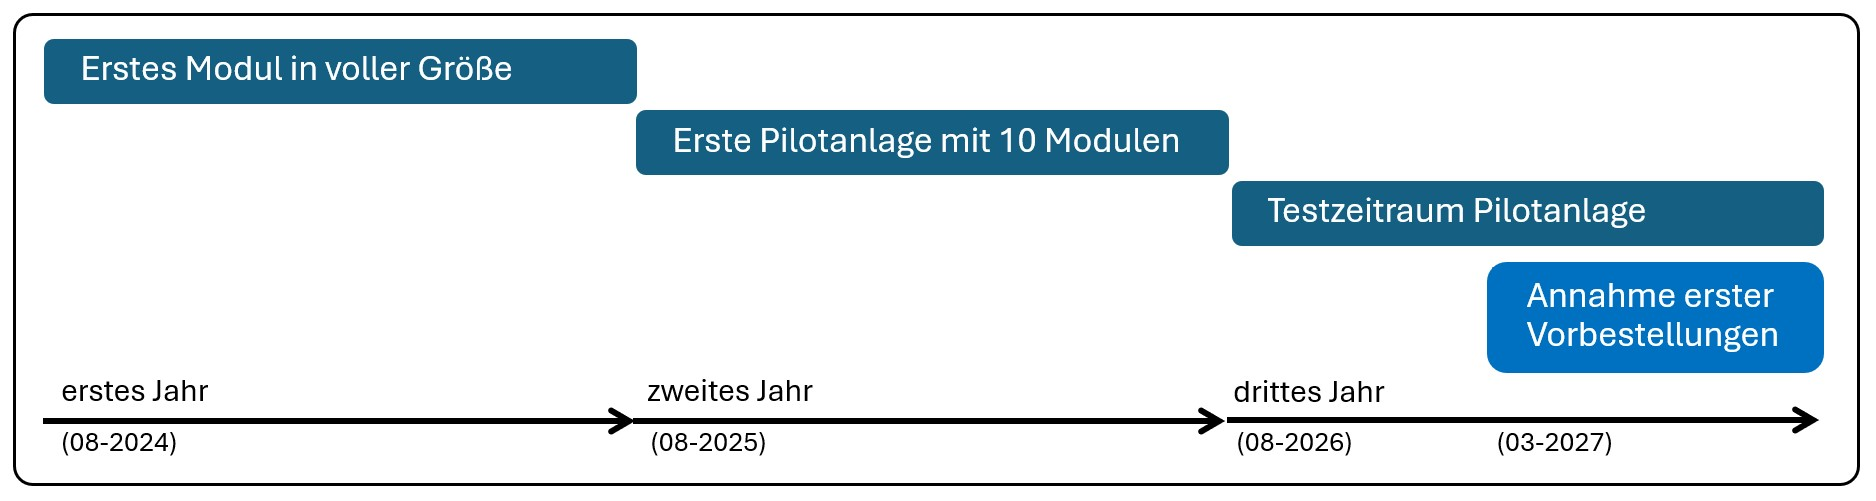
\includegraphics[width=\textwidth]{Zeitlicher-Ablauf.jpg}
        \caption[Übersicht des Arbeitsplans der ersten drei Jahre]{Übersicht des Arbeitsplans der ersten drei Jahre.}\label{fig:zeitliche entw}
    \end{figure}